\RequirePackage[2020-02-02]{latexrelease}  
\documentclass[times]{zHenriquesLab-StyleBioRxiv}
\usepackage{relsize, multirow, xcolor,xargs, placeins}
\usepackage{amsfonts, amsmath, amsthm, amssymb, siunitx} % For math fonts, symbols and environments
\usepackage[normalem]{ulem}
\usepackage[colorinlistoftodos,prependcaption,textsize=tiny]{todonotes}
\usepackage{environ, etoolbox}
\definecolor{sunyGray}{RGB}{131,134,135} \definecolor{sunyBlue}{RGB}{0,76,147}     \definecolor{sunyCyan}{RGB}{0,148,254}                                                            
\newcommandx{\cyansub}[1]{\large\textcolor{sunyCyan} \noindent \textcolor{sunyBlue} {\noindent\textbf{#1}}}                             
% The toggles are initially false  Fig. 
\newtoggle{showFig}
\togglefalse{showFig} \toggletrue{showFig}
\NewEnviron{maybe}[1]{\iftoggle{#1}{\BODY}{}}
\newcommand{\myemph}[1]{\textbf{\textit{#1}}}
\definecolor{sunyWhite}{RGB}{0,0,0}       \definecolor{sunyGray}{RGB}{131,134,135}                                                                                                  
\definecolor{sunyBlue}{RGB}{0,76,147}     \definecolor{sunyCyan}{RGB}{0,158,224}                                                                                                    
\newcommandx{\cnote}[2][1=]{\todo[linecolor=red,backgroundcolor=red!25,bordercolor=red,#1]{Clive: #2}}                                                                              
\newcommandx{\pnote}[2][1=]{\todo[linecolor=blue,backgroundcolor=blue!25,bordercolor=blue,#1]{Paul: #2}}                                                                            
\newcommandx{\tnote}[2][1=]{\todo[linecolor=green,backgroundcolor=green!25,bordercolor=green,#1]{Tade: #2}}                                                                         
\newcommand{\Ga}{\mbox{Ga}} \newcommand{\N}{\mathcal{N}} \newcommand{\E}{\mbox{E}}                                                                                                                                                           
%\newcommand{\V}{\mbox{V}}  \newcommand{\Wi}{\mbox{Wi}}                                                                                                                                                         
\newcommand\eref[1]{{\textbf{\textit{Equation \ref{#1}}}}{}}                                                                                                                        
\newcommand\erefs[2]{\textbf{\textit{Equations \ref{#1} \& \ref{#2}}}}                                                                                                              
\newcommand\fref[1]{\normalsize{\textbf{\textit{Figure \ref{#1}}}}\normalsize{}}                                                                                                    
\newcommand\dref[2]{\normalsize{\textbf{\textit{Figure \ref{#1}#2}}}\normalsize{}}                                                                                                  
\newcommand\sref[1]{\normalsize{\textbf{\textit{Supplemental Figure \ref{#1}}}}\normalsize{}}                                                                                       
\newcommand\tref[1]{\normalsize{\textbf{\textit{Table \ref{#1}}}}\normalsize{}}                                                                                                     
\newcommand\need[1]{\textbf{\textcolor{red}{NEED: #1}}}                                                                                                                             
\DeclareCaptionType[fileext=ext]{Supplementary-Fig}                                                                                                                                 
\newcommand{\unsure}[2][1=]{\todo[linecolor=red,backgroundcolor=red!25,bordercolor=red,#1]{#2}}                                                                                     
\newcommandx{\change}[2][1=]{\todo[linecolor=blue,backgroundcolor=blue!25,bordercolor=blue,#1]{#2}}                                                                                 
\newcommandx{\info}[2][1=]{\todo[linecolor=green,backgroundcolor=red!25,bordercolor=green,#1]{#2}}                                                                                  
\newcommandx{\improvement}[2][1=]{\todo[linecolor=orange,backgroundcolor=orange!25,bordercolor=orange,#1]{#2}}                                                                      
\newcommandx{\thiswillnotshow}[2][1=]{\todo[disable,#1]{#2}}                                                                                                                        
\newcommand\mainpoint[1]{\textbf{\textcolor{blue}{MAINPOINT: #1\\}}}                                                                                                                
\newcommand\question[1]{\textbf{\textcolor{red}{QUESTION: #1}}}                                                                                                                     
\newcommand\minipoint[1]{\smaller{\textbf{\textcolor{purple}{MINIPOINT: #1}}}\normalsize{}}                                                                                         
\newcommand\note[1]{\textbf{\textcolor{red}{\scriptsize{NOTE: #1}}}}                                                                                                                
\newcommand\btext[1]{\textcolor{purple}{Beatrice Draft: \scriptsize{#1}}}                                                                                                           
\newcommand\bmore[1]{\textcolor{purple}{\scriptsize{#1}}}         
\newcommand\pcomment[1]{\textcolor{blue}{\textbf{Issues:} \footnotesize{#1}}}                                                                                                           
\newcommand\tfix[1]{\textcolor{purple}{\textbf{Solutions:} \footnotesize{#1}}}                                                                                                           

\setlength\parindent{0.50cm}
%\leadauthor{Souaiaia} 
\leadauthor{Author} 
\begin{document}
\title{Tail Analysis Indicates Lost Seals} 
\shorttitle{Tails}
%\author[1,\Letter]{Tade Souaiaia}
%\author[2]{Hei Man Wu} 
%\author[2,\Letter,*]{Clive Hoggart} 
%\author[2,\Letter,*]{Paul O'Reilly} 
%\affil[1]{Department of Cell Biology, Suny Downstate Health Sciences, Brooklyn, NY, USA} 
%\affil[2]{Department of Genetics and Genomic Sciences, Icahn School of Medicine, Mount Sinai, 1 Gustave L Levy Pl, NY, NY, USA} 
%\affil[*]{These authors contributed equally to this work} 
\onecolumn \maketitle
\vspace*{-5mm} 
%\begin{corrauthor} \texttt{\small tade.souaiaia\at downstate.edu, clive.hoggary\at mssm.edu, paul.oreilly\at mssm.edu} \end{corrauthor}
\noindent\textcolor{sunyGray}{\rule{17.25cm}{1mm}}
%%%%%%%%%%%%%%%%%%%%%%%%%%%%%%%%%%%%%%%%%%%   END PREAMBLE  %%%%%%%%%%%%%%%%%%%%%
% 
%  PREV: PREAMBLE, NEXT: ABSTRACT
%  PREV: PREAMBLE, NEXT: ABSTRACT
% 
% 
%%%%%%%%%%%%%%%%%%%%%%%%%%%%%%%%%%%%%%%%%%%%%%%%%%%%%%%%%%%%%%%%%%%%%%%%%%%%%%%%%
%%%%%%%%%%%%%%%%%%%%%%%%%%%%%%%%%%%%%%%%%%%   ABSTRACT  %%%%%%%%%%%%%%%%%%%%%%%%%
%%%%%%%%%%%%%%%%%%%%%%%%%%%%%%%%%%%%%%%%%%%%%%%%%%%%%%%%%%%%%%%%%%%%%%%%%%%%%%%%%
\begin{abstract} %\normalsize
\noindent\cyansub{Abstract}$\,$ Complex polygenic traits are typically modeled as the additive sum of 
many variants of limited effect alongside rare risk alleles of substantial penetrence. This distinction 
likely reflects a balance between long-range selection pressure and the limited ability of trait-altering 
mutant alleles to persist over multiple generations.  Identification of individuals with extreme trait values as  
probable carriers of rare high-impact variants has led sequencing strategies to focus on individuals in the tails 
of the trait distribution.  Tail trait values can also result from extreme polygenic burden created by 
recombination and reassortment.  Therefore, to enhance the efficency of sequencing studies, 
it is imperative to be able to discriminate between these different etiologies.  
    
One indicatation that rare variants may play a significant role in the
tails of the trait distribution can be reflected in the reliability of
polygenic risk scores (PRS) in the tails.  If highly penetrant rare
variants not included in GWAS determine the tails of the trait
distribution such individuals will not be assigned appropriate risk
scores.  In this study, we develop a \textit{polygenic
  regression-to-mean} (PRM) statistical test that compares the PRS in
the tails of the trait distribution to expectation PRS under a
polygenic model.  Applying this test to hundreds of traits in the UK
Biobank reveals that the majority of quantitive traits exhibit
significant PRM in one or both tails.

Next we examine whether rare variants in exome studies are enriched in trait tails with significant tail 
regression and demonstrate that such tails are more likely to be under negative selection.  Further examining 
these trait tails we find an association between PRM and other measures of fitness that may be influenced by rare 
variants including the lifetime number of illnesses and still births.  We then compare these 
results to a simulation and find that they match. 

Finally, we assess whether the predictions of a complex trait architecture derived from a conditional sibling model align with the observed diversity 
in the architecture of trait extremes. The concordance between these measures underscores the need to 
consider the role of rare variants in the analysis of trait tails.  The PRS and sibling analyses presented here 
offer valuable tools for the targeted selection of traits and samples likely to harbor de novo or rare 
deleterious alleles and represent an approach that has the potential to significantly enhance the 
effectiveness and design of sequencing studies.
\end {abstract}
\noindent\textcolor{sunyGray}{\rule{17.25cm}{1mm}}
%%%%%%%%%%%%%%%%%%%%%%%%%%%%%%%%%%%%%%%%%%%   END ABSTRACT  %%%%%%%%%%%%%%%%%%%
% 
% 
% 
% 
% 
% 
%  PREV: ABSTRACT, NEXT: INTRO
% 
% 
% 
% 
%%%%%%%%%%%%%%%%%%%%%%%%%%%%%%%%%%%%%%%%%%%%%%%%%%%%%%%%%%%%%%%%%%%%%%%%%%%%%%%%
%%%%%%%%%%%%%%%%%%%%%%%%%%%%%%%%%%%%%%%%%%%   INTRO  %%%%%%%%%%%%%%%%%%%%%%%%%%%
%%%%%%%%%%%%%%%%%%%%%%%%%%%%%%%%%%%%%%%%%%%%%%%%%%%%%%%%%%%%%%%%%%%%%%%%%%%%%%%%
\section*{Introduction} 
%%%%%%%%%%%%%%%%%%%%%%%%%%%%%%%%%%%%%%%%%%% INTRO  PARAGRAPH 1 %%%%%%%%%%%%%%%%%
Genome-wide association studies (GWAS) are instrumental in
understanding the genetic architecture of complex traits.  These
studies typically identify numerous common genetic variants, each of
small individual effect \citep{gwas} that can be used in summation to
make predictions. The idea that these common variants adequately
represent the genetic architecture is supported by evolutionary
theory, which suggests that many human traits (e.g., height, birth
weight) are under stabilizing selection, which reduces the fitness
impact of large-effect variants \citep{v_select}.

A recent hope for advancing personalized medicine is in the potential
of polygenic risk scores to identify high-risk individuals who may
benefit from early interventions, such as adoption of specific
lifestyle regimes or increased screening \citep{bt_7, bt_8, bt_9,
  bt_10}.  However, this strategy will be underpowered when applied to
traits or diseases with reduced PRS in the tail of the distribution
due to reduced common polygenicity. To overcome this problem, the
genetic aetiology underlying the tails of phenotype distributions must
be investigated and better characterized \citep{bt_1}.  Polygenic
prediction models use these common small-effect variants to generate
polygenic risk scores (PRS) whose performance making out-of-sample
predictions is usually evaluated with aggregate estimates like
\emph{variance explained} ($R^2$).  However, new evidence has
suggested that this level of analysis may not be adequate because the
preformance of prediction models is not uniform across the trait
distribution.  This non-uniformity results because the contribution of
small effect common variants relative to highly penetrant rare
variants and the environment is not equal across the trait
distribution \citep{bt_1, bt_2}.

This negative correlation between effect size and minor allele
frequency (MAF) reflects the interplay between long term selection against
extreme trait values and the ability of mutant alleles with
significant effects to escape this trend through chance or short term
environmental changes. Recent or ongoing selection can leave distinct
genetic signatures, such as an enrichment of rare variants in
individuals in the tails of trait distributions during directional or
stabilizing selection. The expectation that individuals with extreme
trait values are more likely to carry rare large-effect variants has
led to strategies that priorize sequencing of individuals in the tails
of the trait distribution \citep{bt_3, bt_4}.  However, tail trait
values can also result from extreme polygenic burden created by
recombination and reassortment, and a more efficient approach would
involve considering more lines of individuals to allow the selection
of individuals with strongest evidence of rare variant architecture
for sequencing.

Here we attempt to distinguish whether the tails of the distribution
of different traits are primarily driven by common polygenicity or by
a more "monogenic-type" architecture \need{monogenic literally means
  single-gene disorder}.  We accomplish this by developing a
statistical test that measures the fit of the polygenic model across
the trait-PRS distribution and identifies non-polygencity in each tail
and applying it to over a \need{thousand} UK Biobank traits (see
\fref{fig:intro}) \need{sentence is too long and "trait-PRS
  distribution" is inaccurate description}.  Next we consider whether
evidence of negative selection exists in a subset of uncorrelated
traits \need{we use all 75 traits, these are not uncorrelated}
and show that the trait tails under negative selection are more
likely to be associated with \need{PRS regression to the mean which
  may imply existence of rare variants}.  We further triangulate
evidence for selective constraint leading to reduced contribution of common
polygenicity in the tails, by testing for the associations between
known measures of fitness and PRS regression to the mean in the tails. \citep{bt_5, bt_6}.

Finally, we assess whether the predictions of a complex
trait architecture derived from a conditional sibling model align with
the observed diversity in the architecture of trait extremes inferred
from population level analyses.


\FloatBarrier \begin{figure}[!h] \centering \begin{maybe}{showFig} 

\includegraphics[trim=0cm 0cm 0cm 0cm, clip, width=\linewidth]{Figures/tailsLogo.pdf} \end{maybe} 
\caption{\footnotesize{\textbf{Placeholder for Schematic}}} \label{fig:intro} \end{figure} \FloatBarrier 
%%%%%%%%%%%%%%%%%%%%%%%%%%%%%%%%%%%%%%%%%%%%%%%%%%%%%%%%%%%%%%%%%%%%%%%%%%%%%%%
%%%%%%%%%%%%%%%%%%%%%%%%%%%%%%%%%%%%   END INTRO %%%%%%%%%%%%%%%%%%%%%%%%%%%%%%%

%%%%%%%%%%%%%%%%%%%%%%%%%%%%%%%%%%%%%%%%%%%%%%%%%%%%%%%%%%%%%%%%%%%%%%%%%%%%%%%%   
%%%%%%%%%%%%%%%%%%%%%%%%%%%%%%%%%%%%%%%%%%%   RESULTS - START  %%%%%%%%%%%%%%%%%
%%%%%%%%%%%%%%%%%%%%%%%%%%%%%%%%%%%%%%%%%%%%%%%%%%%%%%%%%%%%%%%%%%%%%%%%%%%%%%%%
\clearpage \newpage 
\section*{Results} \label{sec:results} 
The traits analyzed in the following section were selected 
from the UK-Biobank categories \textit{Biomarkers}, \textit{Physical Measures}, 
\textit{Touchscreen Questionnaire} and  \textit{Cognitive Tests}.  
Continuous traits from these categories were standardised by regressing 
out the effects of age, sex, and known environmental and technical factors 
and then applying an inverse-normal transformation (see \textit{Methods}).  
Samples were then split in half, GWAS was carried out using Plink \cite{bt_10}, 
and heritability and pairwise genetic correlation was estimated using LDscore \cite{ldsc}.
Applying quality controls for sample size, heritability, skew, and oligogenicity and 
removing strongly correlated traits resulted in the set of 74 traits (see \textit{Methods2}), 
used for POPout associated analyses across the large number of European 
ancestry samples in the UK Biobank. POPout results were replicated three-ways: 
across a subset of repeated measures European ancestry samples in the UK Biobank, 
acorss a subset of non-European ancestry samples in the UK Biobank, and, where applicable, 
across European ancestry samples in the All Of Us Biobank (see \textit{Replication}).



\subsection*{The POPout Test} ~\\ 

Conceptually, POPout occurs when when samples in the tails of the trait phenotype 
distribution have polygenic scores that significantly depart from expectation.  
To quantify this phenomenon we have developed the \textit{POPout test} which regresses
PRS-On-Phenotype to estimate the effect size, direction, and significance of departure from expected PRS 
for individuals in the lower and upper 1\% of the trait distribution (see \textit{Methods}).  

%#29 1 tail #39 2 tail #68 1/2 tail % 90% 
%# defaultdict(<class 'int'>, {'reg': 97, 'pro': 10})

Applying this test to the European ancestry samples in the UK-biobank reveals widespread departure 
from expectation across the 74 traits analysed.  Correcting for multiple tests (5\% false discovery threshold), 
68 of 74 traits have significant POPout effects in one or both tails and that the vast majority (90\%) of these 
effects are positive - i.e. reflect regression to the mean or unexpectedly mild risk scores - 
which is consistent with rare variants of large effects in individuals of the trait tails. 
\dref{fig:prs}{a} illustrates the three broad types of tail effects by plotting trait quantile, 
in 1\% increments, versus mean PRS in the quantile for four index traits: 
\begin{itemize} 
    \item \textit{Ankle Spacing Width} - No POPout Effect in either tail, selected due to highest $h^2$ among such traits, 
    \item \textit{Haemoglobin Concentration} - selected for most significant POPout regression in lower tail only, 
    \item \textit{Red Blood Cell Distribution Width} - selected for most significant POPout regression in upper tail only, 
    \item \textit{Sitting Height} - selected for most significant POPout regression in both tails (minimum value).   
\end{itemize} 
        

\noindent \dref{fig:prs}{b} displays the POPout effects for all traits analyzed, separated into three logical UKB categories, \textit{Biomarkers}, \textit{Physical Measures} 
and \textit{Questionnaire/Cognitive}.  Again positive POPout effects (regression to the mean) predominate, especially with respect to larger effects: 22 tails have 
positive POPout effects greater than 0.25 while none have negative POPout effects less than 0.25.  Here we also observe that POPout regression is 
most common in \textit{Biomarkers} category (79\% of tails) and least common in \textit{Questionnaire/Cognitive} category (43\% of tails). Overall 
we observe a moderate relationship ($R=0.23,Pv=0.018$) between POPout regression and trait heritability, suggesting that POPout regression is 
not driven primarily by environemntal effects.  




  
\FloatBarrier \begin{figure}[!h] \begin{maybe}{showFig} 
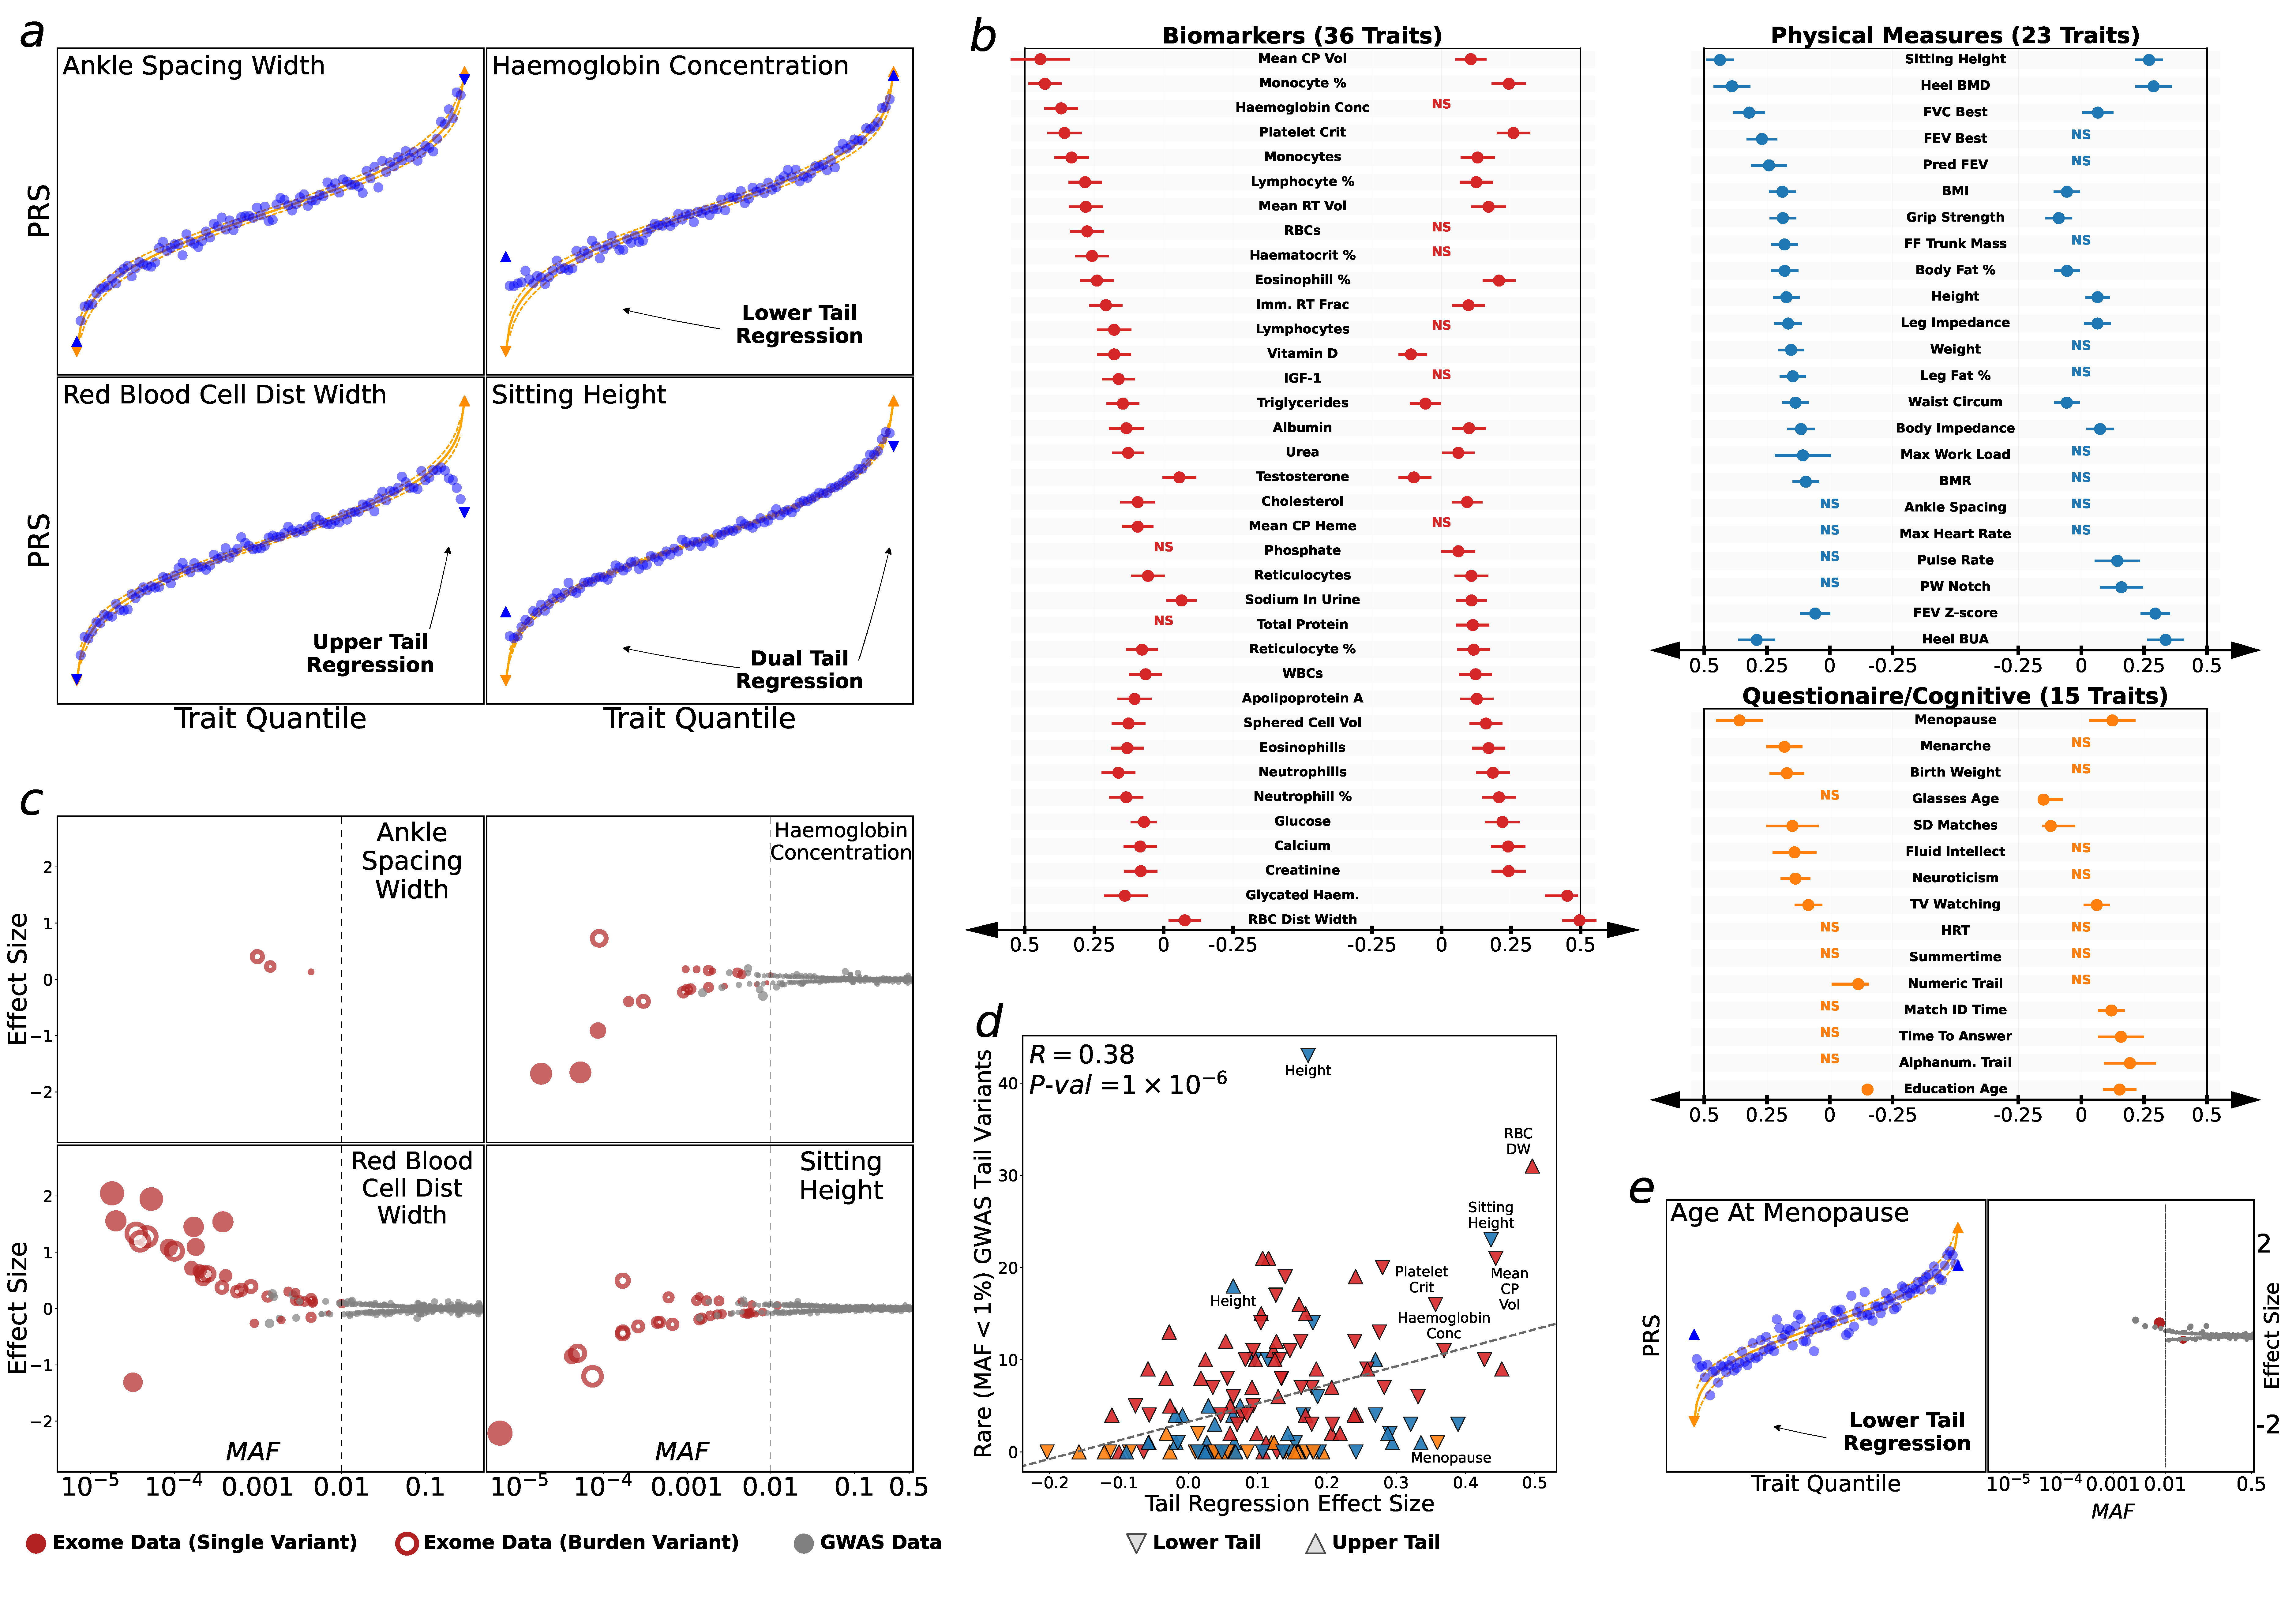
\includegraphics[trim=0cm 0cm 0cm 0cm, clip, width=\linewidth]{Figures/fig2.pdf} \end{maybe} 
\caption{\footnotesize{{\bf Population-level data analyses for rare
      variants of large effect affecting the tails of trait
      distributions.}  \textbf{(a)} PRS quantile (in 1\% increments)
    plotted agaisnt mean trait value in quantile for four traits with
    different PRM results (clockwise: No Tail Regression, Upper Tail, Lower Tail, Dual Tail). 
    \textbf{(b)} PRS-test tail effect sizes and in
    the upper and lower 1\% tails for all 74 traits analyzed. 
    Tail regression effects associated with nominal pvalue $<0.05$ not shown. 
    \textbf{(c)} Trumpet plots (minor allele frequency v effect size) of genome-wide significant
    variants for traits shown in (a). \textbf{(d)} PRM-test tail
    effect sizes plotted against number of genome-wide significant
    variants with MAF<1\% for X traits with overlapping exome sequence
    results. For upper tails positive variant effects are counted and
    for lower tails negative variant effects are counted. Correlation
    and significance calculated using pearson correlation.
    \textbf{(e)} Age of menopause: PRS quantile v trait mean and
    trumpet plot.  }} \label{fig:prs} \end{figure} \FloatBarrier


\subsection*{The Role of Rare Variants} ~\\

\noindent The genetic mechanism proposed to explain POPout involves the confluence 
of genetic selection away from one or both tails, an enrichment of 
rare variants in those tails, and PRS methods that typically restrict 
to common variants (MAF $>1\%$) that suffers in such tails.  Indeed, 
the exclusion of rare variants from PRS has already been shown to 
reduce PRS performance \citep{rares1}. \fref{fig:prs}{c} shows
MAF versus effect size, for genome-wide significant
associations from GWAS \citep{neale} and exome analyses
\citep{backman} of UKB for our four index traits. For \textit{Haemoglobin
Concentration} which exhibits lower tail regression we see a greater
number of rare variants in the lower tail and for \textit{Red Blood Cell
Distribution Width} which exhibits upper tail regression we see a
greater number of rare variants in the upper tail. Sitting height,
which exhibits dual tail regression, has a number of rare variants in
both tails, however, there are more rare variants in the lower tail
where the POPout effect is greatest. For \textit{Ankle Spacing Width} which does
not exhibit POPout in either tail there are just three significant rare
effect variants.  These results are consistent with the hypothesis that
rare variants of large effect that not accounted for in the
common-variant PRS are responsible for tail POPout effects. 

Indeed this relationship holds up across all 74 traits analysed.  In 
In \fref{fig:prs}{d} we observe a small but signficiant relationship
between the magnitude of POPOut regression in the tail and the number of rare
variants in the tail across all 148 trait tails analysed. However, we note that 
while statistically significant, there are multiple traits with signficant 
POPout very significant regression scores for which almost no rare variants 
of substantially large effect have been identified (see \fref{fig:prs}{e}).  
This suggesting that strong selection may result in private variants that cannot be identified using population based
sequencing.

%%%%%%%%%%%%%%%%%%%%%%%%%%% RESULTS-2  %%%%%%%%%%%%%%%%%%%%%%%%%%%%%%%%%

\FloatBarrier \begin{figure}[!h] \begin{maybe}{showFig} 
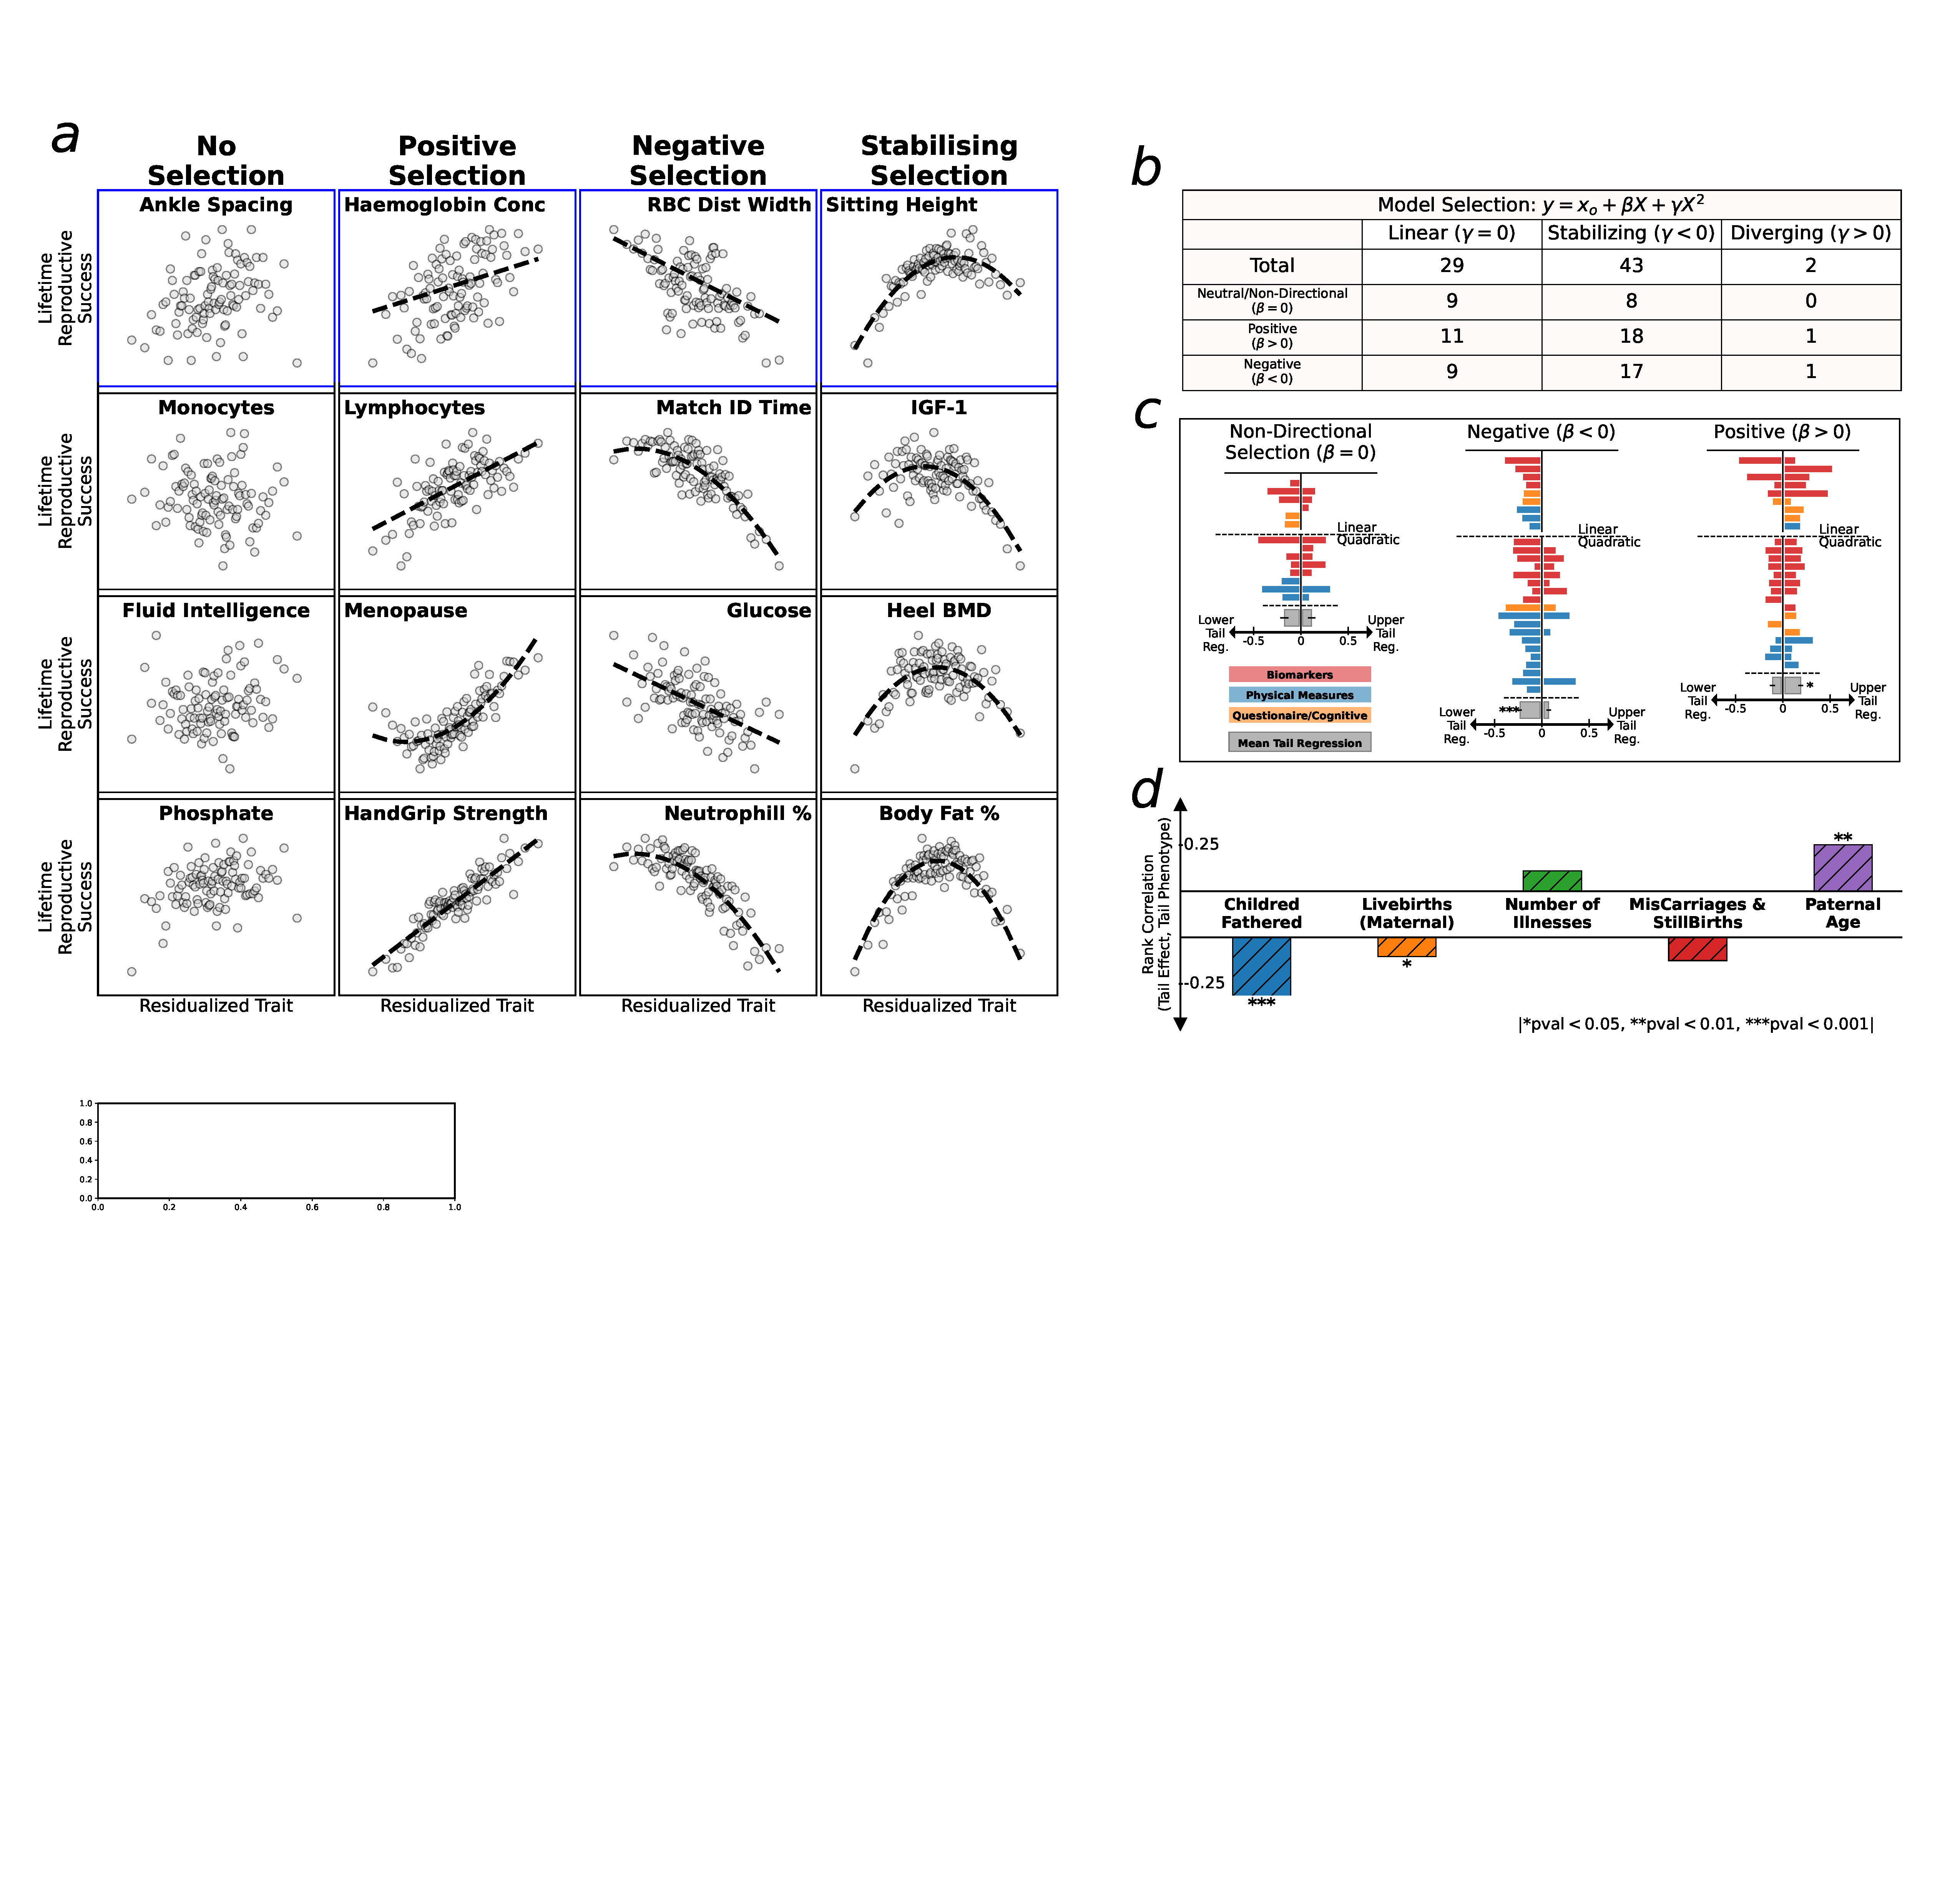
\includegraphics[trim=0cm 0cm 0cm 0cm, clip, width=\linewidth]{Figures/fig3.pdf} \end{maybe} 
\caption{\footnotesize{{\bf Selection analyses in real and simulated
      data.} \textbf{(a)} Residualised trait value plotted against
    relative lifetime reproductive success for 16 example traits.
    Best model fit to the data, selected by BIC considering all models
    with and without linear and quadratic terms, are shown by dashed
    lines. Model selected by BIC used to classify selective pressure
    acting on the traits. \textbf{(b)} PRS-test effect size shown by
    trait selection category, with PRS-test effect size meta-analysis
    for each category. \textbf{(c)} Spearman rank correlation between
    four proxy measures of fitness and PRS-test effect size. For each
    fitness measure correlation was calculated between the mean of the
    fitness measure in individuals in the upper and lower 1\% tails
    and PRS-test effect size for the corresponding tail across 74
    traits in UKB passing QC. Fitness measures were standardised by...
    \textbf{(e)} \need{Coming Soon} Trumpet plots (minor allele
    frequency v effect size) for simulated data without and with
    selection. All variants are included in the plot. \textbf{(e)} PRS
    quantile (in 1\% increments) plotted agaisnt mean trait value in
    quantile in simulated data without and with selection. PRS
    calculated from all variants with MAF>1\%.
  }} \label{fig:evo} \end{figure} \FloatBarrier

\subsection*{The Impact of Selection on PRM} ~\\
Using adjusted lifetime reproductive success \citep{v_select,
  v_select2} as a proxy for selection we classify (see Methods - LRS)
each trait with respect to whether it is under \emph{Stabilizing,
  Positive, Negative, or Neutral/Disruptive} selection (these results
are in agreement with a more comprehensive sex-specific analysis (See
\fref{fig:vishy}).  The majority of traits analyzed here (55 of 75)
are classified as under stabilizing selection which is characterized
by lower fecundity for individuals with traits values in either tail
of the trait distribution. Stabilizing selection may be the result of
general fitness favoring the trait mean or the result of sex specific
selection that averages to produce this relationship \citep{v_select}.
Eight traits were classified as being under positive selection and
seven traits were classified as being under negative selection.  We
also classified four traits as under neutral selection (no signficant
relationship with LRS) and one trait as divergent/disruptive selection
where fecundity is higher in both tails that at the mean of the
distribution (\fref{fig:evo}{a}).  We find a significant relationship
between selection classification and PRM classifition
(\fref{fig:evo}{b}), whereby traits under stabilizing selection are
enriched in "Dual Tail Regression" ($p< 2.5 \times 10^{-5}$), traits
under positive selection are enriched in "Lower Tail Regression
($p < 2.4 \times 10 ^{-4}$), and traits under negative selection are
enriched in "Upper Tail Regression ($p < 0.024$).  Focusing on each
tail separately we find an even stronger relationship insofar as the
in the 118 trait tails which exhibit PRM, the tail is selected against
110 times (93\%) while in the 32 tails which do not exhibit PRM the
tail is only selected against 16 times (50\%) ($pv < 0.001$).



\subsubsection*{Tail Fitness} ~\\ 
\noindent In addition to \emph{lifetime reproductive success}, we
analyzed four measures of fitness that are likely to be associated
with reduced fitness and rare variant or \emph{de novo} etiology.
Here, we note that under the hypothesis that rare variants under
negative selection are responsible for PRM, we predict that trait
tails with large effect PRM will have lower average \emph{lifetime
  reproductive success} and higher average numbers of \emph{Still
  Births} and \emph{Miscarriages}.  Additionally, traits tails with
large effect PRM are predicted to have more standarized illnesses
because both result from large effect variants, although it is
possible that downstream effects of illnesses results in extreme trait
values.  Finally, if paternal age is associated with more \emph{de
  novo} mutations \citep{pat} it should also be associated with PRM.

In \fref{fig:evo}{c} the rank correlation for the average tail fitness
measure and the PRM effect size across the trait tails is shown.  We
observe that the direction of rank association is in line with the
rare-variant hypothesis in every case, although the association
between PRM and the number of miscarriages and paternal age are not
significantly associated.


\subsubsection*{Simulating Selection (Anil's Result)} ~\\  
In \fref{fig:evo}{d} we confirm this result using a simulation (see \emph{Methods}) 
where we simulate many generations of stablilzing selection, after which the ratio 
of contribution to heritability by rare variants goes up and PRM is observed. 

%%%%%%%%%%%%%%%%%%%%%%%%%%% RESULTS-3  %%%%%%%%%%%%%%%%%%%%%%%%%%%%%%%%%

\subsection*{\emph{Replication in Siblings}} ~\\
Discordance between siblings in the tails of the trait distribution is
indictive non-polygenic inheritance \cite{avi}. Furthermore, excess
trait concordance between siblings can be indicative of shared
Mendelian effects \cite{t_sibs}. \fref{fig:sib}{a} illustartes the
expected impact of polygenicity, de novo, and Mendelian rare variants
within sibling pairs. Expected sibling pair concordance under
polygenicity can be used to test for (1) excess discordance between
siblings in tails of trait distribution, indicative of de novo
mutations of large in one sibling and (2) excess concordance between
siblings in tails of trait distribution, indicative of shared
Mendelian effects \cite{t_sibs}. These tests are derived from the
conditional sibling distribution under polygenicity, this distribution
also allows heritability to be estimated \cite{t_sibs}.

Applying this model to the sibling data in the UKB to estimate $h^2$, 
we find a correlation between snp h2 and sibling h2 \fref{fig:sib}{b}.  
In our index traits we use this model to infer the presence of rare 
variant architecture in the tails and find that lower tail discordance 
in \emph{Haemoglobin Concentration}, upper tail discordance in 
\emph{Red Blood Cell Distribution Width} and dual ail discordance 
in \emph{Sitting Height}, all of which match the result from our PRM 
test.  Overall we find a significant relationship between our sibling 
test pvalue and the pvalue from our PRM-test \fref{fig:sib}{d}. 



\FloatBarrier \begin{figure}[!h] 
  \begin{maybe}{showFig} 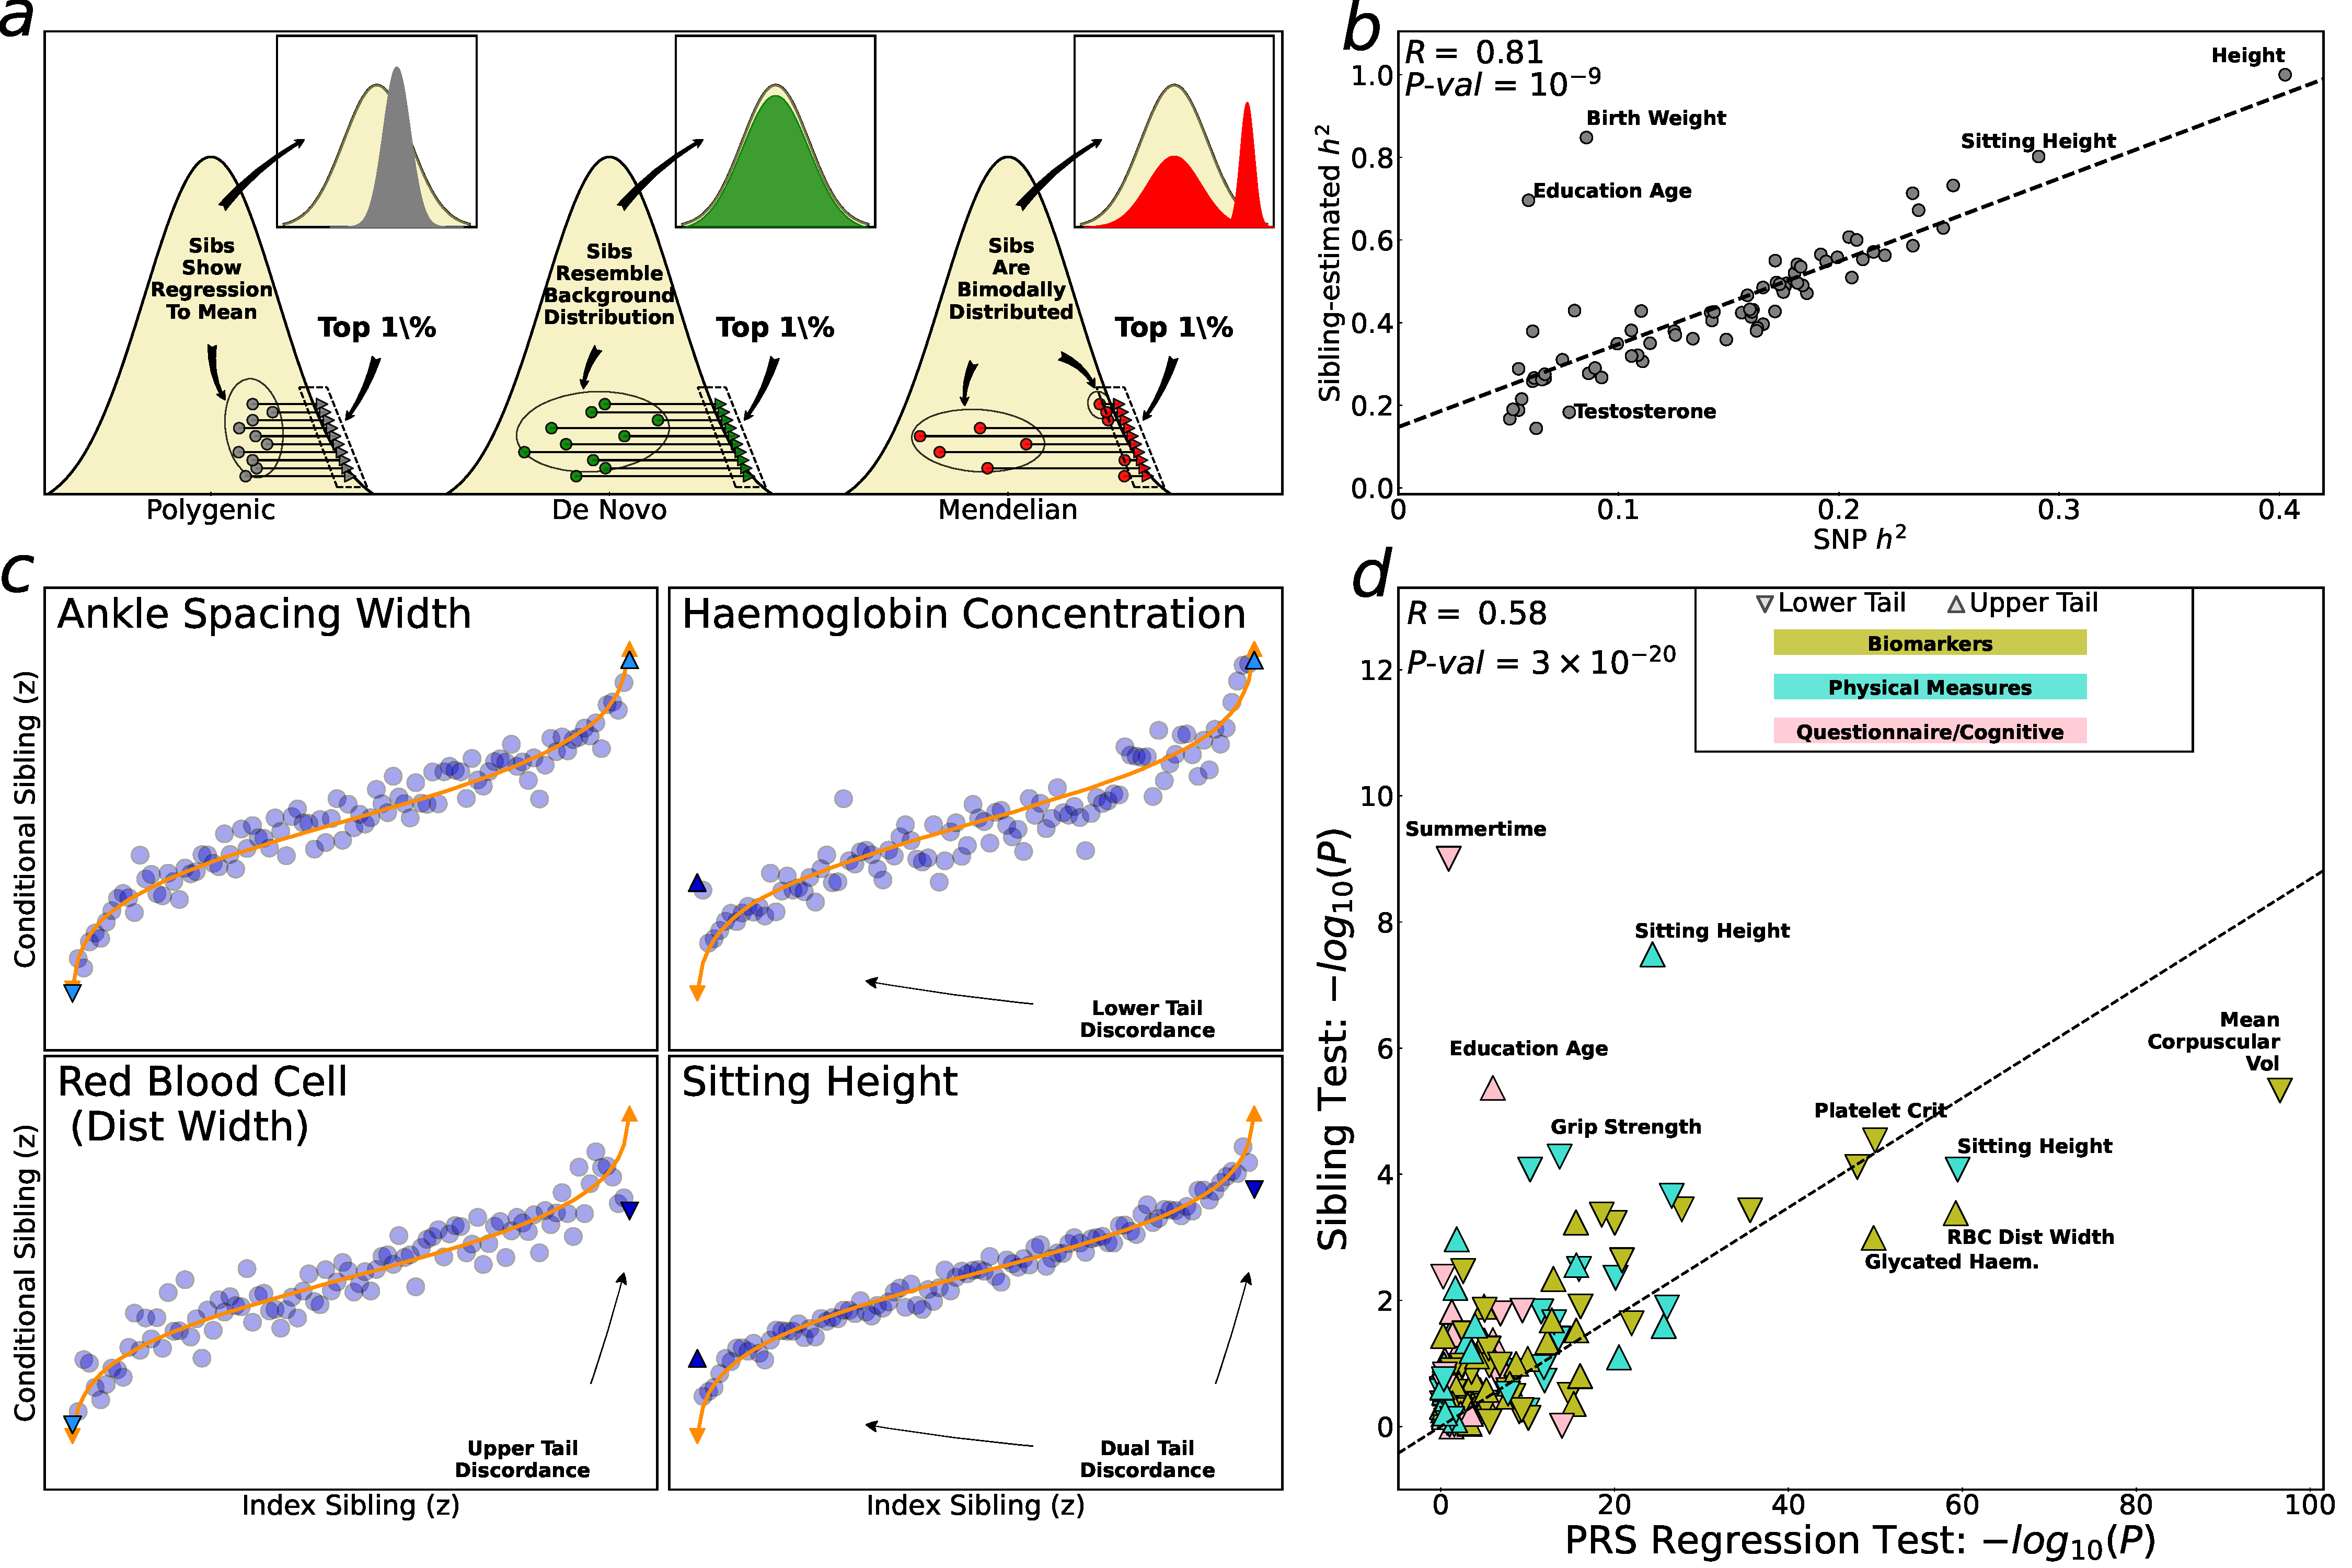
\includegraphics[trim=0cm 0cm 0cm 0cm, clip, width=\linewidth]{Figures/fig4.pdf} \end{maybe} 
  \caption{\footnotesize{{\bf Sibling analyses for rare variants of
        large effect affecting the tails of trait distribution.}
      \textbf{(a)} Schematic of relationship of sibling trait values
      under polygenicity, de novo variants of large effect in one
      sibling and rare inherited variant of large effect,
      Mendelian. \textbf{(b)} LDscore regression SNP
      heritability plotted against heritability estimated from sibling
      pair trait similarity using European UKB samples.  \textbf{(c)}
      Index sibling trait quantile (in 1\% increments) plotted agaisnt
      mean trait value of conditional sibling in quantile for four
      traits with different types of PRS tail regression. \textbf{(d)}
      PRS-test P-values plotted against sibling de novo and Mendelian
      test meta analysis P-values on $-\log_{10}$ scale for upper and
      lower tails of \need{X} traits. Correlation calculated using
      pearson correlation.}}
    \label{fig:sib} \end{figure} \FloatBarrier


%%%%%%%%%%%%%%%%%%%%%%%%%%%   RESULTS-4 Replication  %%%%%%%%%%%%%%%%%%%%%%%%%%%%%%%%%
\subsection*{\emph{Replication}} ~\\

We performed three \emph{flavours} of replication. 

\begin{enumerate}                                                                               
\item \textbf{Repeated Subsets of The Target Data:} Assess the reliability of our PRM-test in smaller samples
\item \textbf{Non-European Ancestry Inviduals in UKB:}  PRM replication across ancestry (within biobank) 
\item \textbf{European Ancestry Individuals in All Of Us:} PRM replication across biobank (within ancestry) 
\end{enumerate} 


\subsubsection*{Bootstrap Analysis using Target Subsets} ~\\ 
\noindent To assess the performance of our PRM-test using smaller samples 
we re-sampled small subsets of our target populations, and performed our 
PRM-test on these subsets. In \ref{fig:rep}{d} we notice that even the 
correlation of effect sizes was approximately 0.70 even when the subset 
size was only 5k, however concordance in discovery was poor at these levels. 


\subsubsection*{Out of Sample Replication} ~\\
\noindent The correlation between PRM effect-sizes was greater in the
UKB Non-European Ancestry data despite smaller sample sizes, although
the number of true positives identified was lower (underpowered).
This suggests that even if PRS isn't portable across ancestry, that
regression to the mean is portable and in fact may be even more than
portable.





\FloatBarrier \begin{figure}[!h] \begin{maybe}{showFig} \includegraphics[trim=0cm 0cm 0cm 0cm, clip, width=\linewidth]{Figures/fig5.pdf} \end{maybe} 
  \caption{\footnotesize{{\bf PRS test replication results in UKB
        repeated measures, UKB non-European samples, All of Us
        European ancestry.} \textbf{(a)} PRS quantile (in 1\%
      increments) plotted agaisnt mean trait value in quantile for
      four traits with different types of PRS tail regression for
      discovery and replication cohorts.  \textbf{(b)} PRS-test effect
      size in discovery and replication cohorts across 25 traits
      measured and passing PRS-test quality control in all cohorts.
      \textbf{(c-e)} PRS-test effect sizes estimated in UKB European
      ancestry discovery samples and replication cohort: \textbf{(c)}
      UKB European ancestry sample repeated measures, \textbf{(d)} UKB
      non-European ancestry samples and (e) AllofUs European
      ancestry. Triangles shaded relative to the replication sample
      size for the trait. Pearson correlation shown.
      samples. \textbf{(f)}....}  } \label{fig:rep} \end{figure}
\FloatBarrier



\FloatBarrier \begin{figure}[!h] \begin{maybe}{showFig} \includegraphics[trim=0cm 0cm 0cm 0cm, clip, width=\linewidth]{Figures/fig6.pdf} \end{maybe} 
  \caption{\footnotesize{{\bf Analysis of POPout Impact on PRS 
        Prediction} Repeated for Three Traits.  
        \textbf{(a)} POPout Figure - Phenotype on PRS. 
        \textbf{(b)} PRS on Phenotype Figure. 
        \textbf{(c)} Cumulative POPout Distributions show non-informative tails. 
        \textbf{(d)} Pseudo Case/Control Analysis: Denoting the upper/lower tail 
        (10\%, 5\%, 1\%, 0.5\%) as case status, log-odds relative to the middle 
        PRS-quantile is calculated for each of twenty PRS quantiles. 
        }  } \label{fig:pred} \end{figure} \FloatBarrier


%%%%%%%%%%%%%%%%%%%%%%%%%%%%%%%%%%%%   END RESULTS %%%%%%%%%%%%%%%%%%%%%%%%%%%%%%%%%
%
%
%
%%%%%%%%%%%%%%%%%%%%%%%%%%%%%%%%%%%%%%%%%%%%%%%%%%%%%%%%%%%%%%%%%%%%%%%%%%%%%%%%%%%%
%%%%%%%%%%%%%%%%%%%%%%%%%%%%%%%%%%%%%%%%%%%   DISCUSSION - START  %%%%%%%%%%%%%%%%%%
%%%%%%%%%%%%%%%%%%%%%%%%%%%%%%%%%%%%%%%%%%%%%%%%%%%%%%%%%%%%%%%%%%%%%%%%%%%%%%%%%%%%
\clearpage \newpage
\section*{Discussion} \label{sec:discussion} In this study, we propose
the use of PRS Regression-to-the-Mean (RM) Test as a way to identify
traits that are enriched for rare or de novo – more “monogenic-type”
effects (MTE) in extreme.  We applied this method to a list of
quantitative traits available in UKB. In addition to genotype data, we
also incorporated the rich source of UKB information including the
sibling data (Sibling RM Test), and paternal age (Paternal Age Test)
and number of children (Fecundity Test) into our analyses.  We found
directional consistency in most of the tests performed, providing
converging evidence for the feasibility of using PRS as a strategy to
identify traits with potential MTE.  In our analyses, the PRS RM test
can be used to identify both the “polygenic” and “MTE” event, we
hypothesize that for a highly polygenic trait, samples with extreme
trait values (ETV) are expected to have extreme PRS
correspondingly. Deviation from the expectation may suggest samples at
the extreme tails are enriched for MTE that are under selection. Our
results show significant correlation in the ranking traits from least
to most evidence of common polygenicity in the tails of their
distributions between the PRS RM test and Fecundity test. Furthermore,
the results of the PRS RM test are supported by the Sibling RM test of
which we use the sibling phenotype data to investigate the common
polygenicity in different traits.  Sib-pairs are expected to have
similar trait value under the influence of common polygenicity. On the
other hand, if the ETV in sib A is contributed by de novo mutations,
we expect sib B to be discordant phenotypically. An alternative
explanation for discordant phenotype in sib-pairs could be due to the
non-shared environment factors with large effect.

The striking concordance between these measures underscores the need
to consider the role of rare variants in the analysis of trait tails.
The PRS and sibling analyses presented here offer valuable tools for
the targeted selection of traits and samples likely to harbor de novo
or rare deleterious alleles and represent an approach that has the
potential to significantly enhance the effectiveness and design of
sequencing studies.

One major limitation of these tests is that they are highly sensitive
to measurement errors. Measurement errors would result in the same
PRS/ sibling departure at the extreme ends, because the PRS is no
longer reflective by one’s phenotypic measurement. In addition, both
the PRS RM and sibling RM Test cannot distinguish between large effect
mediated by environmental factors and MTE. For example, if a person
with extremely low levels of LDL but normal PRS can be caused by
malnutrition.  Therefore, collection of the associated environmental
factors and the corresponding adjustment becomes vital to alleviate
this problem when applying these tests. Moreover, these tests are only
applicable to quantitative traits, more work is needed to develop for
testing binary outcome.  In this study, we identified traits with
evidence to be influenced by MTE at the trait tail(s), however, we did
not identify or confirm the corresponding de novo mutation. Despite
the lack of parent-offspring trios which is essential for the
identification of de novo mutations, it is technically challenging to
define a list of candidate genes and variants for every trait we
investigated. Further investigation is warranted to validate this
finding.  In conclusion, we propose a novel way of using polygenic
risk score to look for evidence of de novo/ rare mutations. This can
be used as a method to identify traits that are more likely influenced
by de novo mutations, and select samples who are more likely carry de
novo mutations, potentially maximizing the power of a sequencing
study. This method can be applied to any traits with continuous
measure such as age of onset, disease severity and rate of disease
progression.

%%%%%%%%%%%%%%%%%%%%%%%%%%%%%%%%%%%%   END DISCUSSION %%%%%%%

%%%%%%%%%%%%%%%%%%%%%%%%%%%%%%%%%%%%%%%%%%%%%%%%%%%%%%%%%%%%%%%%%%%%%%%%%%%%%%%%%%%%%%   
%%%%%%%%%%%%%%%%%%%%%%%%%%%%%%%%%%%%%%%%%%%   METHODS - START     %%%%%%%%%%%%%%%%%%%%
%%%%%%%%%%%%%%%%%%%%%%%%%%%%%%%%%%%%%%%%%%%%%%%%%%%%%%%%%%%%%%%%%%%%%%%%%%%%%%%%%%%%%%
\clearpage \newpage 
\section*{Methods} 
%%%%%%%%%%%%%%   METHODS 1- DATA PROCESSING %%%%%%%%%%%%
\subsection*{Data Processing} ~\\
\vspace*{-0.5cm} 
\subsubsection*{UK Biobank Genetic Data} ~\\

\pcomment{
\begin{itemize} 
\item  More specifics on the numbers. 
\item  Explain ancestry clustering more specifically (which ancestries?
\item  What PC values chosen?). Nobody could repeat this accurately as written. 
\item  Some loose language in places. Several places where citations needed e.g. “recommended by the UK Biobank team.” i
\item  Need some better context - e.g. In the primary analyses in unrelated individuals (Figures 2, 3, 5)...
\item  In the analyses performed on siblings (Figure 4)... 
\item  Not sure if Mixed ancestry results needed anymore?
\end{itemize}
}

The UK Biobank (UKB) is a prospective cohort study of approximately
500,000 participants recruited across the United Kingdom from 2006 to
2010 \citep{ukb}. Phenotype data of anthropometric, biological and
lifestyle measures was collected at baseline and follow-up surveys, with
further linkage to health and disease record data. The genetic dataset
consists of 488,377 samples genotyped at 805,426 SNPs.

To determine population ancestries, 4-means clustering analysis was
conducted on the first two Principal Components (PCs) of the genotype
data. Samples were then projected onto 1000 Genomes PCs to determine
ancestry, resulting in 461,931 European, 11,074 South Asian, 7,935
African, 2,585 West Asian, 2,550 East Asian, 1,619 and admixed
samples.

Subsequent to clustering, standard quality control (QC) procedures
were applied independently to each ancestry cluster. SNPs with a minor
allele frequency $<$ 0.01, genotype missingness > 0.02, or
Hardy-Weinberg equilibrium test $P$-value $< 10^{-8}$ were
excluded. Samples exhibiting high levels of missingness or
heterozygosity, inconsistencies in genetic-inferred and self-reported
sex, or displaying aneuploidy of the sex chromosomes were removed in
accordance with recommendations from the UKB data processing team
\citep{ukb_qc}.  For the analyses on the general population, a greedy
algorithm was employed to remove related individuals that maximises
sample retention while removing all third-degree relatives (kinship
coefficient > 0.044) \citep{erase}.  After this QC 411,949 unrelated
individuals remained.  Primary analyses were performed on the over
387,235 unrelated European samples that comprised the largest ancestry
cluster. Replication analyses were performed on the remaining 24,476
samples that comprised multiple non-European ancestries.

For the sibling analyses, sibling pairs were selected by first
identifying first-degree relatives, defined as those with kinship
coefficient within the range 0.177 and 0.354 (expected value for
siblings is 0.25) to account for the expected variation in within-pair
similarity \citep{sib1}. Only individuals of European ancestry were
included in the sibling analyses. The proportion of SNPs with zero
identity-by-state (IBS0) was used to distinguish sibling pairs from
parent-offspring pairs, since parent–offspring pairs have
IBS0$\approx$0 across the autosomes. It has been shown in the UKB that
there is good separation between pairs of first degree relatives at
IBS0=0.00112 \citep{sib1} and, thus, sibling pairs were selected as
those exceeding this threshold, giving a total of 17,289 sibling pairs
of European ancestry for analysis.


\subsubsection*{Quantitative Trait QC} ~\\

\pcomment{
\begin{enumerate} 
\item Seems a bit unusual to describe the QC, then the
  residualisation/normalisation, and then some further QC steps on the
  untransformed data. Is this the best order?
\item I think the reduction from 151 to 92 traits due to rg<0.99
  cut-off is likely to raise alarm bells - how many more would’ve been
  lost if you’d used 0.98, 0.95, 0.9 instead?
\item There are a lot of P-values reported in the paper dependent on a
  test of many traits.. but if those are highly correlated then the
  overall P-value reported will be inflated. We’ve talked about this
  before I know but isn’t this still a problem!?
\end{enumerate} 
}

\tfix{
\begin{enumerate} 
\item I don't know.  But basically Clives PRM-QC finds non-linearities 
    but we know our normalization can hide them, so it does make sense to
    be conservative here. 
\item Filtering on Clives QC first and doing genetically correlations 
last (as we should), it hardly makes a difference, I changed it to 0.95 
and gave some numbers that should calm alarm bells. 
\item They are not highly correlated - but I think we have done 
enough in the methods to make people calm.
\item This does need to be talked about in the discussion - the 
whole point of the paper is TAILS, and the tails are 
nothing like the main part of the distribution, so highly 
correlated body doesn't mean much about the tails. 
\end{enumerate}
}

\subsubsection*{Individual level QC}
After genetic QC, individuals on insulin and pregant women at baseline
were removed from all trait analyses. For blood count and biochemisty
traits, individuals on statins and other cholesterol lowering drugs
were removed. \need{Cancer patients traits were removed from the
  following traits analyses.... Individuals on beta-blockers were
removed from from pulse rate traits.}


\subsubsection*{Class Selection} 

I removed: 
\begin{enumerate} 
    \item \textit{Raw acceleromter statistics} 
    \item \textit{Population Characteristics, Local Environment} (Air Pollution) 
    \item \textit{MRI and NMR} 
    \item \textit{Diet by 24-hour Recall} (unreliable)  
    \item \textit{Derived OCT measures} 
\end{enumerate} 



\subsubsection*{Trait selection}
Quantitative traits were selected for analysis as those with at least
10 distinct values and for which the top two modal trait values
combined comprised less than 50\% of the trait distribution. To ensure
that our analyses were well-powered, traits with heritability
$h^2<5\%$ (estimated by LD score \citep{ldsc} applied to publicly
available UKB GWAS summary statistics \citep{neale}) and $<$50,000
unrelated samples with observed trait measures were removed, this gave
175 traits.




\subsubsection*{Trait QC}
Trait specific QC was then performed, first, to ensure extreme
outliers did not impact results, trait values more than six
standard deviations from the mean were removed. To minimise the effect
of environmental risk factors on the results, trait values were then
standardised by applying a linear regression model to each trait, with
covariates for age, sex, recruitment centre, genotyping batch, and the
first 40 genetic principal components [WHAT ABOUT AGE2 ETC AND THE
FULL REGRESSION THAT WAS PERFORMED??].

Subsequently, traits with skew $>2$ and multimodal residuals (dip-test
\citep{dip} $P$-value for unimodality $<$ 0.05) were
removed. Residualised trait values were then normalised by inverse
normal transforming the rank of the residuals to give normally
distributed traits for analysis.  To ensure
that the selected traits were polygenic, traits for which a single
variant explains more than 0.5\% of trait variance
($r^2 > 0.5\%$) were removed.  To ensure that the traits analysed were
meaningly different from each other, we calculated pairwise genetic
correlations using LDscore\cite{ldsc}. THE REMAINING SENTENCES OF THIS
PARAGRAPH ARE A MESS AND NEED FIXING. Sixty one traits did not have a
pair with $r_g>98\%$ and were retained for analyses. Additionally, 10
traits had a single almost identical match (eg: "Standing Height"
(ID:50) and "Height Measured Prior to Imaging" (ID:12144)), and in
these cases the trait with greater sample size was prioritised.  The
other 52 traits were part of larger clusters of genetically similar
traits, the largest of which related to measurements related to of
body-mass (eg: body fat percentage, leg mass, arm mass, etc) and heel
bone mineral density.  Using the same data maximisation algorithm used
to select unrelated individuals \citep{erase}, 11 such traits were
then selected, resulting in a set of 77 genetically different traits
for analysis.

\subsection*{Genome-wide association analyses and PRS estimation in UKB}
European UKB samples were split randomly into 50\% base and 50\%
target data sets. GWASs were applied to the base data using PLINK-1.9
\citep{bt_10} applying a linear additive model to the standardised
trait values. PRScice-2(v2.3.4) \citep{prsice} was applied to the GWAS
summary statistics of each trait with fast-scoring to select the most
predictive P-value threshold within the target data. Individual risk
scores were calculated for UKB target samples.

\subsection*{Replication}
\subsubsection*{Bootstrap Analysis using Target Subsets}
Our 75 QC-validated traits were required to have at least 100k total
samples.  In the target sample (half the total), after outlier removal
our QC-validated traits had between of 50,085 and 185,362 (average
142k) target samples.  To explore whether our PRM-test results
replicate with smaller sample sizes, we repeatedly sampled subsets of
between 5k and 50k target samples and performed our PRM-test on these
subsets.  For each value between 5k and 50k (counting by 5k) we
performed 100 trials across each of the 150 trait tails and calculated
the \textbf{(1)} relative accuracy (true and false positives and
negatives) relative to our full dataset (FDR 5\%) and \textbf{(2)} the
linear and the rank correlation of for the regression effect size
across all the tails.

\subsubsection*{Repeated measures replication} ~\\
\need{Details...}

\subsubsection*{Replication in All of Us Cohort} ~\\
All of Us is a biobank of individuals of multiple ancestries from
across the United States of America. Traits matching those analysed in
the primary UKB analysis were identified through an initial database
search and were then interrogated manually to determine if trait
descriptions were sufficiently similar.  All of Us provide ancestry
categories, corresponding to definitions used within gnomAD, the Human
Genome Diversity Project, and 1000 Genome, \need {XX,XXX} European ancestry
individuals were extracted for analysis. There were too few
individuals of non-European ancestry for sufficient replication power.
\need{Trait values were normalised by...} \need{Genotype data....}

%%%%%%%%%%%%%%   METHODS 2- DATA ANALYSIS %%%%%%%%%%%%

\subsection*{Data Analysis} ~\\
\vspace*{-0.5cm} 
\subsubsection*{The PRS-regression tail test}~\\
The PRS-test first applies a regression of PRS on trait values where
both the PRS and trait are standardised to have standard deviation of
1. For each trait, the residuals from the regression are split
into quantiles according to the trait distribution and two-tailed
t-tests are applied to test whether the residuals are significantly
different from zero.  The tests were applied to individiuals in the top
and bottom 1\% of the trait distribution. The effect size in each tail
is defined such that a positive effect is indicative of regression to
the mean in both the upper and lower tails as follows
\[
\frac{1}{n}\sum_i^n |{f(y_i)}| - |{PRS_i}|
\]
where $f(y)$ is the predicted PRS from the regression given trait
value $y$ and $n$ is the number of observations.

\subsubsection*{The PRS-regression test QC}~\\
An additional trait QC was applied to ensure the robustness of the
PRS-test by testing the residuals of samples in the middle of the
trait distribution for departure from the null of zero mean.
Specifically, for each trait, two-sided t-tests for zero mean were
applied to the residuals assigned in each of the middle 80 centiles of
the trait distribution. Traits were deemed to fail QC if the smallest
P-value was significant at a Bonferroni-corrected level of 0.05 (P
$\le$ 0.05/80).

%\subsubsection*{Empirical PRS-regression test}~\\
%A robust empirical P-value for deviation in trait tails was calculated
%as follows: for each centile of trait one-sided t-tests for residuals
%less than and greater than zero were calculated.  The P-value for
%regression to the mean in the upper tail was calculated from the rank
%of the tests for residuals significantly less than zero and the lower
%tail empirical P-value from the greater than zero tests. The tests
%were performed on all 1,121 continuous traits in UKB.

\subsubsection*{Trumpet plots} ~\\
Trumpet plots show the effect sizes and MAF of independent genome-wide
significant variants. Common variants (MAF$>$1\%) were selected as the
most significant variant (P$\le 5\times 10^{-8}$) in 1Mb windows from
publicly available GWAS summary statistics generated using UKB samples
of European ancestry \cite{neale}. Exome sequencing associations from
the analysis of UKB European ancestry samples were downloaded
\cite{backman}. Results are plotted for the most significant
deleterious, missense or predicted loss of function variants in each gene
(P$\le 2.18\times 10^{-11}$, one association per gene). Genome-wide
significant burden associations are shown where no single variant
within the gene is genome-wide significant.

\subsubsection*{Sibling concordance tests}~\\
The conditional distribution under polygenicity of an individual's
trait value given their siblings trait value is predicted by theory
\cite{t_sibs}
\begin{equation} p(s_2 \mid s_1 ) \sim \N\left(\frac{1}{2}s_1h^2,
1-\frac{h^4}{4}\right) \label{math:S2givenS1}
\end{equation}
where $s_1$ and $s_2$ denote the index and conditional-sibling trait
values respectively and $h^2$ is the trait heritability. Rare
large-effect variants can lead to deviations from this distribution,
particularly in the tails.  Specifically, rare large-effect variants
within families, {\em Mendelian effects}, will result in excess
concordance between siblings when they both inherit the effect
variant. Conversely, a large effect {\em de novo} mutation in one
sibling will result in excess discordance. The sibling test for {\em
Mendelian} effects applies a binomial test for a greater than
expected number of sibling pairs both lying in a defined quantile of
the tail of the trait distribution by calculating the following
z-statistic
\begin{align*}
z&=\frac{r-n\pi_0}{\sqrt{n\pi_0(1-\pi_0)}}
\intertext{where $n$ is the number of index siblings in the quantile $q$ 
under test, $r$ is the number of siblings pairs both in $q$ and $\pi_0$ 
is the expected proportion of sibling-pairs in the quantile under polygenicity}
\pi_0&=\frac{1}{n}\sum_{i\in A_q} \left( 1 - \Phi \left(
\frac{\Phi^{-1}(q)  - \frac{s_1^{(i)}
h^2}{2}}{\sqrt{1-\frac{h^4}{4}}} \right)\right)
\end{align*}
where $A_q$ is the set of index siblings in trait quantile $q$,
$\Phi$ is the normal normal cumulative density function, $\Phi^{-1}$
is its inverse and $n$ is the number of sibling pairs.

The sibling test for {\em de novo} effects constructs a z-statistic
for the distance between index siblings in the tail of the trait
distribution and their conditional siblings as follows
\begin{align*}
  z&=\frac{\sum_{i\in A_q}s_2^{(i)}-\frac{1}{2}s_1^{(i)}h^2} {\sqrt{n(1-\frac{h^4}{4})}}
\end{align*}
For index siblings in the lower and upper tails the alternative
hypotheses of $H_1: z>0$ and $H_1: z<0$ are tested respectively. For
further details see Souaiaia et al \citep{t_sibs}.  Heritability $h^2$ 
required for the {\em Mendelian} and {\em de novo} tests is estimated 
from the sibling pairs by taking the maximum likelihood of $h^2$ 
under the null hypotheses of both tests
\begin{equation*} \log \mathcal{L} \propto -n\log\left(1 -
    \frac{h^4}{4}\right) - \frac{1}{1-\frac{h^4}{4}} \sum_{i=1}^n
  \left( s_{2}^{(i)} - \frac{s_1^{(i)} h^2}{2}
  \right)^2
\end{equation*}

The sibling meta P-value was calculated by combining P-values from the
{\em Mendelian} and {\em de novo} tests using Fisher's method to give
a $\chi^2$ statistic with 4 degrees of freedom,
\begin{align*}
    \chi^2_4 = -2(\log(p_{Mendelian}) + \log(p_{de novo}))
\end{align*}


%%%%%%%%%%%   LRS   %%%%%%%%%%%%
\subsection*{Selection Analyses}
\subsubsection*{Relative Lifetime Reproductive Success} ~\\
The number of offspring is recorded in the UKB for both females and
males, fields \textit{2734} and \textit{2405} respectively.  Following
the methodology of Beauchamp \citep{v_select2}, samples were split
into four birth cohorts (1934-42, 1943-48, 1949-55,
1956-65). Individual relative
lifetime reproductive success, $Y_{rLRS}$, was then calculated by
dividing the number of offspring of each individual by the cohort
mean. Following Sanjak et al \citep{v_select}, the presence and
direction of selective pressure acting on traits was determined by
fitting the following regression model:
\begin{equation}
Y_{rLRS} = \beta_o + \beta z + \gamma z^2 \label{math:LRS}
\end{equation}
where $z$ denotes the residualised and normalised trait values and
$\beta$ and $\gamma$ are linear and quadratic regression parameters.

The Bayesian information criteria (BIC) was used to select the best
fitting model for each trait from which the selective pressure acting
on trait was inferred. If the selected model did not include a linear
or quadratic parameter, no selection was inferred, here rare variant
enrichment is not expected in either tail. If the selected model
included only the linear parameter $\beta$, negative selection was
inferred if $\beta<0$ and rare variant enrichment is expected in the
upper tail, while positive selection was inferred if $\beta>0$ and
rare variant enrichment is expected in the lower tail. If the selected
model included only the quadratic parameter $\gamma$, with $\gamma<0$,
stabilising selection is inferred and the mean trait value in the
population is at its optimum and rare variant enrichment is expected
in the both tails. Divergent selection is implied by $\gamma>0$, in
this scenario rare variant enrichment is not expected in either
tail. If the selected model included both linear and quadratic
parameters with $\gamma<0$ stabilising and directional selection was
inferred, in which the optimal trait value is within the range of the
population values but is not the population mean. With
$\beta<0$ it is inferred that selection is causing the trait mean to
decrease and greater rare variant enrichment is expected in the upper
tail. Conversely, with $\beta>0$ it is inferred that selection is
causing the trait mean to decrease and greater rare variant enrichment
is expected in the lower tail.  If $\gamma>0$ then rare variant
enrichment is not expected in either tail.

Concordance between inferred selection and the PRS test for traits
classified as exhibiting both stabilising and directional selection
was tested by a Fisher exact test, comparing binary categories
$\beta<0$ / $\beta>0$ with PRS-test effect size greater in upper /
lower tail.  For traits classified as no selection, directional
selection and stabilising selection, concordance with PRS-test used
the PRS-test classifications of no / lower / upper / dual tail
regression. Fisher exact tests were constructed separately for
negative, postive and stablising selection for enrichment in the
expected PRS-test classification, lower / upper / dual respectively,
by collapsing the other categories, traits classified as exhibiting
both stabilising and directional selection were excluded from these
tests.

%%%%%%%%%%%   TAIL FITNESS   %%%%%%%%%%%%
\subsubsection*{Association between PRS-test and proxy measures of fitness}~\\
Four proxy measures of fitness were considered. (1) Standardised
self-reported non-cancer illnesses (UKB trait field 2002) determined
by the residuals of a regression with covariates for age, sex and
recruitment centre. (2) Number of miscarriages (trait field
38290). (3) Number of still-births (trait field 3839). (4) Paternal
age at birth.

Association between these measures and the PRS-test was tested as
follows.  The mean value of the four proxies of selection was
calculated separately in the upper and lower 1\% of the trait
distribution, association was then tested by Spearman's rank
correlation across all trait tails of the mean tail values for each
proxy and the PRS-test effect size.

\subsubsection*{Simulating Stabilizing Selection using SLiM} ~\\
Using SLiM v4.0 (1), we simulated a quantitative polygenic trait under
a standard Wright-Fisher (WF) model of stabilising selection. First a
population of N=10,000 diploid individuals of 1Mb was simulated to
equilibrium (10N generations) with a constant mutation of
$2.36\times 10^{-8}$ per base pair (bp) and recombination rate of
$10^{-8}$ per bp under neutrallity. Mutations were assigned effect
sizes simulated from a gamma distribution with shape parameter 0.186
and mean 0.01026 and subsequently multiplied by -1 with probability
0.5 to give a symmetrical effect size distribution. This distribution
has been used previously to simulate genetic effects in humans and
reflects a prior belief in a small number of large effects and many
small effects \cite{anil3}. Individual trait values were determined by
the sum of all genetic effects.

After neutral genetic diversity was achieved (10N generations),
stabilising selection on the trait was introduced for 1N
generations through a Gaussian fitness function
\begin{equation} 
  f_t(x) = 1 + \frac{1}{\sqrt{2\pi\sigma^2}} \exp\left\{-\frac{(x-\mu)^2}{2\sigma^2}\right\}
\end{equation}
where $x$ is the phenotype of an individual at generation $t$, $\mu$
and $\sigma$ are the trait mean and standard deviation at the start of
selection (i.e., $t=10N$). Stabilizing selection was simulated for a
further 1N generations after the 10N burn-in generations.

Simulation data was collected by logging, at each generation, the
phenotypic mean and standard deviation of the population, statistics
of mutations present in the populations, including allele frequencies
and effect sizes, and the mutational profile of each individual. To
investigate the contributopn of low-frequency variants and mimic a PRS
based on common variants, a second genetic value was calculate using
only variants with $MAF > 1\%$.

\clearpage \newpage
\bibliography{refs}
\clearpage \newpage



\section*{Supplement} \label{sec:supplement}



\section*{Addendum 1: PRS Prediction} \label{sec:supplement}

In this manuscript we have focused on polygenic regression to the mean, which can be observed when plotting 
the average PRS score (Y) across the quantiles of the trait distribution (X) (see \fref{fig:sup1}{a}).  
Importantly, when we visualize the relationship between the average phenotype (Y) across the quantiles 
of the PRS distribution the effect isn't visible in mean (see \fref{fig:sup1}{o}) and can only be observed 
in variance (see \fref{fig:sup1}{r}) because non-polygenic influences on the trait appear independent from 
the PRS distribution*** and thus are uniformly distributed. (*THIS IS IMPORTANT -suggests non-additive). 

Here we provide an example of the effect that PRM can have on disease prediction using the continuous trait 
RBC distribution width (see \fref{fig:sup1}{x}), namely that, a PRS score in the bottom 5\% of the PRS 
increases the probability of being in the bottom 50\%, bottom 25\%, bottom 5\%, bottom 1\%, and bottom 0.1\% 
of the trait distribution by 1.4, 1.8, 2.8, 3.2, and 3.5 times.  Consider the other side of the trait 
distribution, a bottom 5\% PRS score reduces the probability of trait score in the top 50\% (0.595), 
top 25\% (0.495), top 5\% (0.62), and top 1\% (0.855) but does not reduce the probability of being 
in the top 0.1\% (1.2x). 

Continuing, a PRS score in the top 5\% of the PRS, increses the risk of being in the 
top 50\% (1.4), top 25\% (1.7), top 5\% (1.78), top 1\% (1.4x), but does not increase the risk 
of being in the top 0.1\% (0.816). 


To summarize, for this trait the predictive value of polygenic scores is: 

\begin{itemize} 
\item Low PRS increases probability of very low trait scores 
\item Low PRS descreases probability of moderately high trait scores 
\item High PRS increases probability of moderately high trait score but not very high trait score
\end{itemize} 

\noindent Consequently, if disease state occurs for the top 0.1\% of the trait distribution, PRS is not 
predictive. 



\FloatBarrier \begin{figure}[!h] \begin{maybe}{showFig} 
\includegraphics[trim=0cm 0cm 0cm 0cm, clip, width=\linewidth]{Figures/checkplot_30070.pdf} \end{maybe}
\caption{\footnotesize{\textbf{Sample and SNP Workflow}}} \label{fig:sup1} \end{figure} \FloatBarrier

\clearpage \newpage

\section*{Addendum 2: QC Figures} \label{sec:supplement}

\FloatBarrier \begin{figure}[!h] \begin{maybe}{showFig} 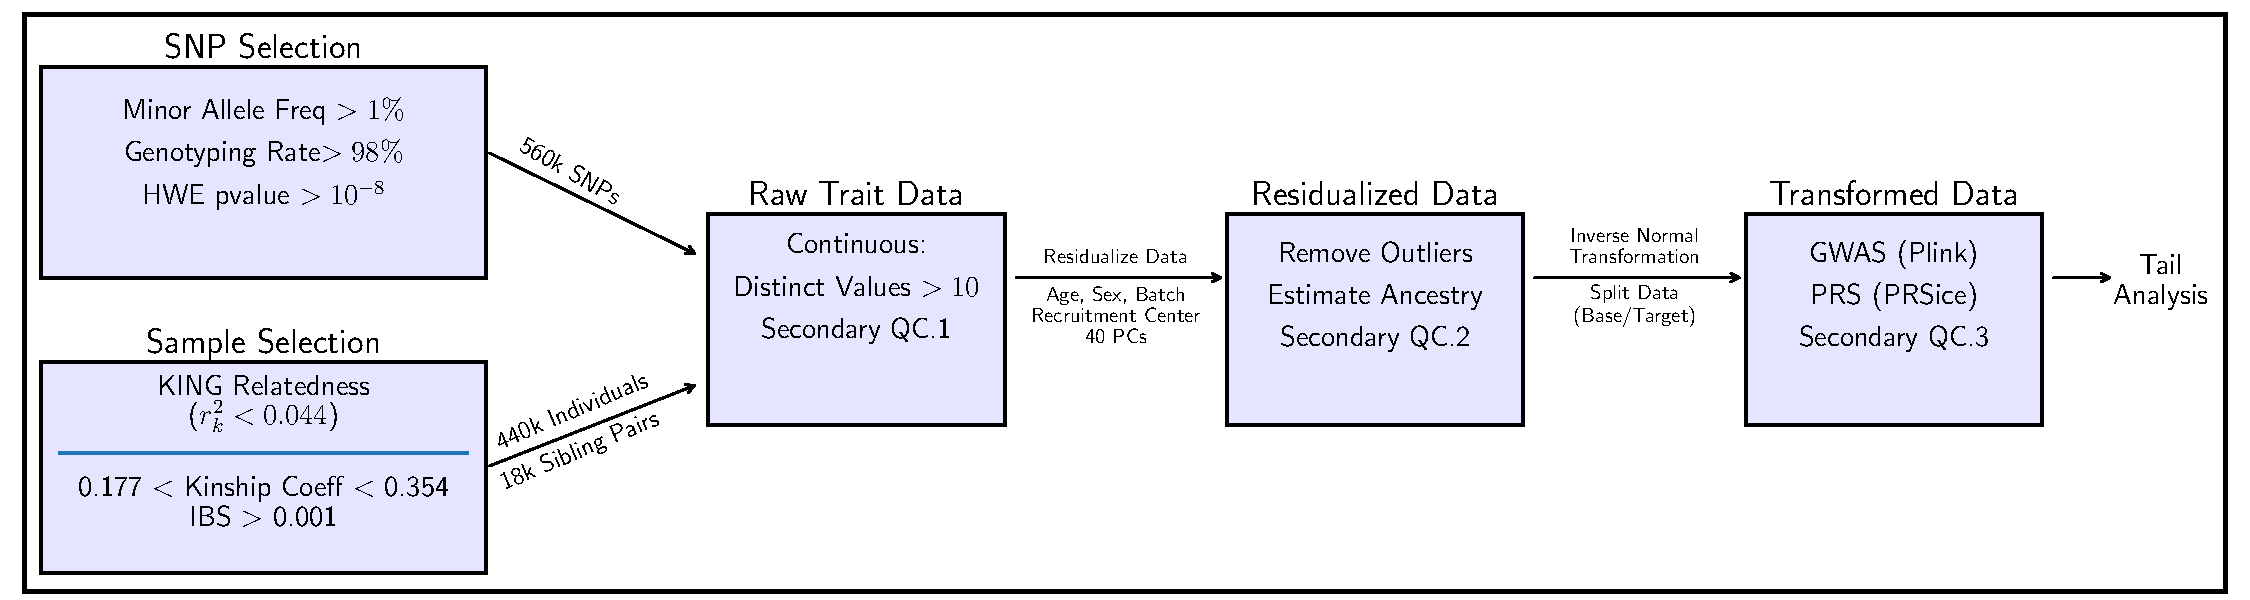
\includegraphics[trim=0cm 0cm 0cm 0cm, clip, width=\linewidth]{Figures/methodFlow.pdf} \end{maybe}
\caption{\footnotesize{\textbf{Sample and SNP Workflow}}} \label{fig:qcFlow} \end{figure} \FloatBarrier



\begin{figure}[!ht] \centering \begin{maybe}{showFig} 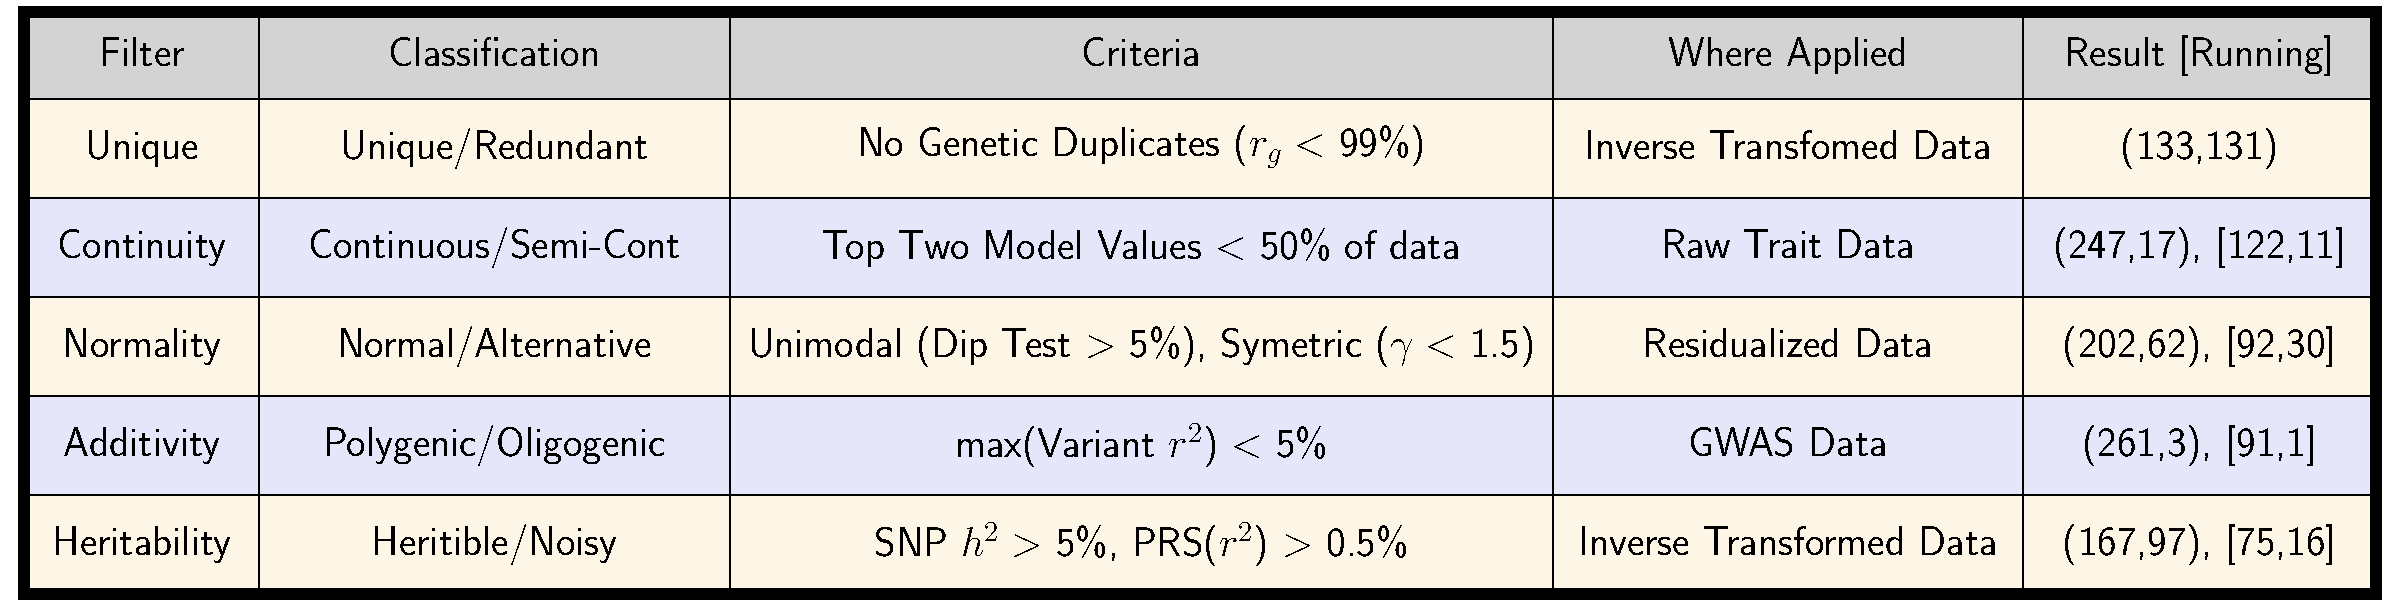
\includegraphics[trim=0cm 0cm 0cm 0cm, clip, width=16.5cm]{Figures/qctable.pdf} \end{maybe} \label{fig:m2} \caption{\scriptsize Secondary QC} \end{figure} 
\clearpage \newpage

\section*{Addendum 3: Lifetime Reproductive Success} \label{sec:supplement}

\FloatBarrier \begin{figure}[!h] \centering \begin{maybe}{showFig} 
\includegraphics[trim=0cm 0cm 0cm 0cm, clip, width=16.5cm]{Figures/vishtable.pdf} \end{maybe} 
\caption{\footnotesize{\textbf{Comparison of Selection Estimates}}} \label{fig:vishy} \end{figure} \FloatBarrier 

\clearpage \newpage
%
%
%
%
%
%
\clearpage \newpage
\end{document}
